\subsection{CryptoImg}
A paper published in 2009 by Ziad, et al. implements privacy-preserving image processing using \textit{CryptoImg}, a library for the Open Source Computer Vision Library (OpenCV)~\cite{bradski_opencv_2000} which implements various homomorphic encryption and image processing routines using the Paillier homomorphic cryptosystem~\cite{ziad_cryptoimg:_2016}. The \textit{CryptoImg} library assumed a client-server model wherein a client requests image processing operations from a server. A client first encrypts a digital image and sends the image securely to a server, which then operates on the encrypted image without revealing its contents. The resulting image is sent back to the client, which decrypts the image to recover the desired output.
\begin{figure}[!ht]
    \centering
    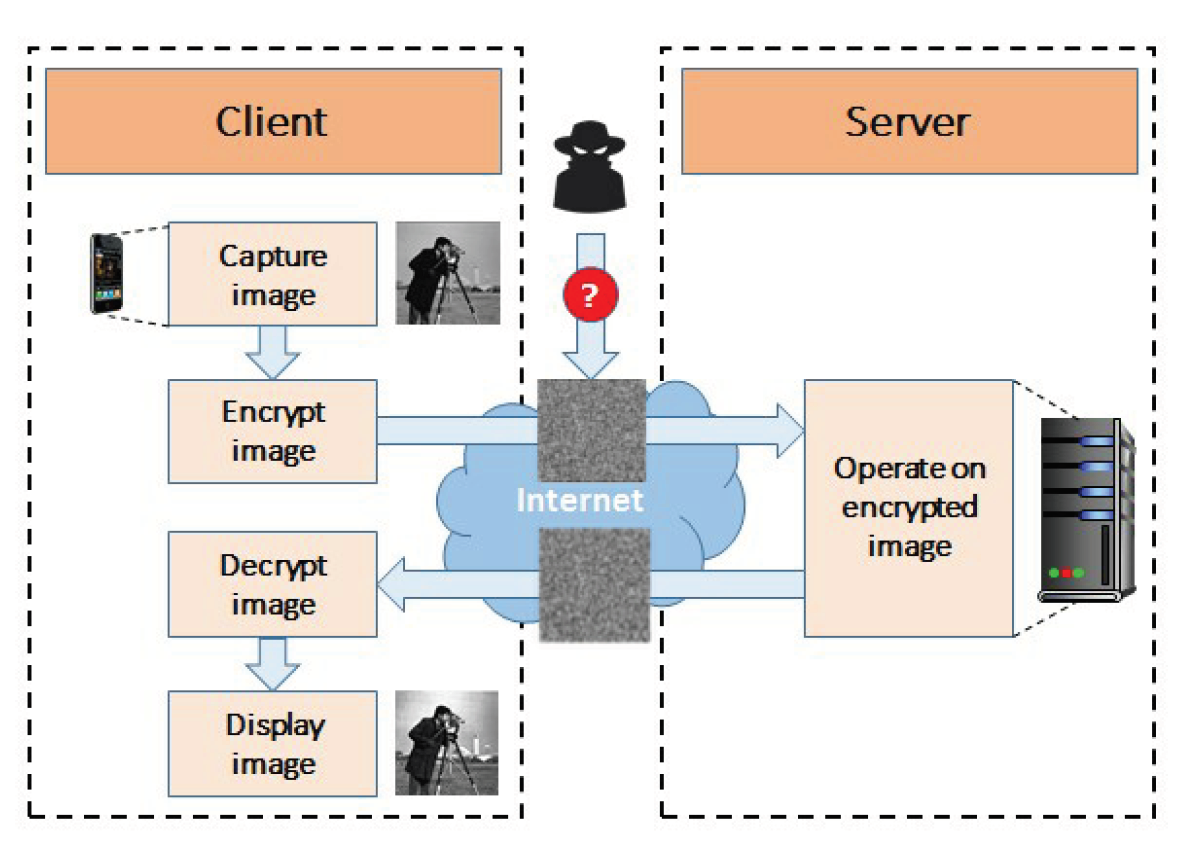
\includegraphics[width=0.4\textwidth]{figures/ClientServerModel.png}
    \caption{Client-server architecture used by \textit{CryptoImg} \cite{ziad_cryptoimg:_2016}}
    \label{fig:clientserver}
\end{figure}

The \textit{CryptoImg} library implemented the following image processing operations: image negation, brightness adjustment, spatial filters (for noise reduction, edge detection and sharpening), morphological operations, and histogram equalization.

% For image negation and spatial filters, the protocols specified by \textit{CryptoImg} allow all image processing operations to be performed on the server. However, due to limitations in the Paillier cryptosystem, the protocols presented for morphological operations and histogram equalization require both the client and the server to perform image processing calculations, although the server performs a significant portion of the processing.

Ziad, et al. also showed experimental results establishing the relatively slow performance of image operations under a homomorphic cryptosystem. For instance, while sharpening and applying a Sobel filter each take less than a second when applied to a $512\times 512$ plaintext image, when applied to an encrypted image, sharpening required at least 238.257 seconds, and applying the Sobel filter required at least 147.567 seconds \cite{ziad_cryptoimg:_2016}.


% We now discuss several limitations in the \textit{CryptoImg} study which we focus on for our research. First, the \textit{CryptoImg} library was limited in the image intensity transformations it implemented. We propose additional protocols to support more computationally intensive intensity transformations.
% Second, the \textit{CryptoImg} library only considered the Paillier cryptosystem. We consider testing the performance of other homomorphic cryptosystems, which differ in their processing time and supported operations.

% Convert to single table
\subsection{Image Intensity Transformations}
We represent a digital image $R$ as an $M \times N$ matrix of pixel intensity values, each value in the range $\left[0, L-1\right]$, for some positive integer $L$. We denote with $R(x,y)$ the entry at the $x$th row and $y$th column of a matrix $R$.
An intensity transformation on an image $R$ can be defined as a function $T$ which is applied to every pixel $r$ in $R$.
The \textit{CryptoImg} library implemented two types of linear intensity transformations: image negation and brightness control. An image negation transformation is defined as
\begin{equation}
    T\left(r\right) = L-1-r,
\end{equation}
which results in an image similar to a photographic negative~\cite{gonzalez_digital_2008}.
A brightness control transformation with parameter $v$ is defined as
\begin{equation}
    T\left(r,v\right) = r+v.
\end{equation}
The above transformations are linear in terms of the input $r$, and are thus simple to implement under a homomorphic cryptosystem.

In this study we extend the range of intensity transformations to non-linear transformations. Two common non-linear image transformations are the logarithm transformation and power-law transformation~\cite{gonzalez_digital_2008}.

The logarithm transformation is used to enhance dark pixels or increase the dark details of an image by mapping low intensity values to a wider range of values~\cite{gonzalez_digital_2008}. This has the general formula
\begin{equation}
    T\left(r\right) = c \log\left(1 + r\right)
\end{equation}
where $c$ is a constant.
The power-law transformation is a family of transformations that have the form
\begin{equation}
    T\left(r\right) = c r^{\gamma}
\end{equation}
where $c>0$ and $\gamma > 0$.
A power-law transformation can calibrate the operation of many image capture and output devices such as cameras, printers and displays in a process called \textit{gamma correction}.
% This ensures reproducibility and accuracy of images being displayed by digital output devices~\cite{gonzalez_digital_2008}.

To implement non-linear intensity transformations using addition and multiplication in a homomorphic system, it is necessary to approximate the logarithm and exponential functions, which may result in higher computational overhead. An applicable approximation for the logarithm may be found in \cite{pcsc-paper}. 
% In our software library implementation, we investigate methods required to approximate the logarithm and power functions. 
Non-linear intensity transformations such as the logarithm transformation have applications in intensity normalization \cite{oravec_illumination_2010}, which is used in some facial recognition algorithms to account for differences in lighting which make facial recognition difficult.